\documentclass[journal]{IEEEtran}
\usepackage{amsmath,amsfonts}
\usepackage{algorithmic}
\usepackage{array}
\usepackage[caption=false,font=normalsize,labelfont=sf,textfont=sf]{subfig}
\usepackage{textcomp}
\usepackage{stfloats}
\usepackage{url}
\usepackage{verbatim}
\usepackage{graphicx}
\graphicspath{{./figures/}}
\hyphenation{op-tical net-works semi-conduc-tor IEEE-Xplore}
\def\BibTeX{{\rm B\kern-.05em{\sc i\kern-.025em b}\kern-.08em
    T\kern-.1667em\lower.7ex\hbox{E}\kern-.125emX}}
\usepackage{balance}
\usepackage{biblatex}
\usepackage{listings}
\lstset{
    basicstyle=\footnotesize,
    numbers=left,
    xleftmargin=2em,
    stepnumber=1,
    showstringspaces=false,
    tabsize=1,
    breaklines=true,
    breakatwhitespace=false,
    frame=single
}
\usepackage{float}
\usepackage{hyperref}

\addbibresource{references.bib}

\begin{document}
\title{The automated detection of fraudulent peer-to-peer transactions in massively multiplayer online economies}
\author{Hayley Davies - 1902055}

\maketitle
\footnote{Source code for all algorithms is availible on GitHub: \url{https://github.com/cdgamedev/dissertation}}
\footnote{Source \LaTeX is availble on Falmouth GitHub: \url{https://github.falmouth.ac.uk/Games-Academy-Student-Work-22-23/1902055-comp3xx-dissertation}}

\begin{abstract}
Massively Multiplayer Online games are a hugely popular and successful subsection of the gaming industry. These games allow players to trade items within the game, but some players choose to buy and sell in-game items for real-world money, known as Real Money Trading. This leads to people preferring to buy from illicit sources rather than through the game itself, resulting in a loss of revenue for the developers. Additionally, this practice enables people to make money through methods such as botting, account theft, or cheating.
\end{abstract}

\begin{IEEEkeywords}
Anomaly Detection, Massively Multiplayer Online, Real Money Trading
\end{IEEEkeywords}


\section{Introduction}
\IEEEPARstart{R}{eal-Money} Trading (RMT) is the practice of buying and selling virtual items and currency within massively multiplayer online (MMO) video games. This practice often violates the games' Terms of Service or Code of Conduct\cite{AmazonGamesCOC}\cite{SquareEnixCOC}, and as a result, players who engage in RMT are often at risk of being banned from the game. RMT has negative effects on the game's economy and community, and it is therefore discouraged by game developers and players alike.

\section{Literature Review}
\subsection{Anomaly Detection for RMT}
\noindent Anomaly detection is a technique used to help address the issue of RMT in MMOs\cite{Tao2019}\cite{Ahmad2009}. By using computers to flag in-game transactions automatically for human review, it is possible to identify and prevent RMT activity in a way where humans don't have to analyse the all the data manually by hand. Preventing RMT helps to protect the game's economy and maintain a fair and balanced playing experience for all players. However, it is important to note that the effectiveness of this approach will depend on the specific details of the game and the methods used for detecting anomalies.

Fujita et al. propose a method for addressing the issue of RMT in MMO games, which involves identifying suspects, verifying their involvement in RMT activity, and banning their accounts\cite{Fujita2011}. They also classify RMT players into three categories: 
\begin{itemize}
    \item \textit{Sellers} are those who sell the virtual property to players for real-world money.
    \item \textit{Earners} acquire virtual property (currency and items) from non-player characters (NPCs) and real players.
    \item \textit{Collectors} convey virtual property from earners to sellers.
\end{itemize}

Fujita et al. manually classified a set of players and then used an algorithm proposed by Newman and Girvan\cite{Girvan2002} to extract communities and further identify players. They ranked players based on the number of times they traded currency, the number of trades they made in total, and the total volume of currency traded.

Fujita et al. argue that RMT is harmful to both the game's economy and its players, as it is often associated with other illicit activities such as cheating, botting, and account theft. RMT can also drive away legitimate players who become frustrated with the problems it causes, and it can discourage new players from joining the game\cite{Sifa2021}. Overall, Fujita et al. believe that RMT is a serious issue that needs to be addressed to protect the integrity and health of MMO games. Han et al. and Sifa et al. back up Fujita's claims adding that "cheating in MMOs often reduces the shelf life of the game" by causing people to abandon it\cite{Han2022}\cite{Sifa2021}.

\subsection{Types of Anomaly}
\noindent Anomalous data can typically be categorized in three different ways\cite{Ahmed2016}\cite{Bhuyan2013}. These categories are:
\begin{itemize}
    \item \textbf{Point Anomaly} where a data point is unusually out of range.
    \item \textbf{Contextual Anomaly} (or collective anomaly\cite{Song2007}) where sometimes, a data point which seems anomalous is actually within range depending on a varying factors.
    \item \textbf{Collective Anomaly} is where multiple data points are out of range, but when considered individually, are not out of range.
\end{itemize}
Understanding these categories can help researchers identify and address potential issues in their data. By detecting anomalies, it may be possible to uncover hidden patterns or trends and improve the accuracy and reliability of data-driven systems and models.

\subsection{Machine Learning}
\noindent Due to the nature of anomaly detection is often done with Machine Learning (ML) algorithms\cite{Omar2013}\cite{Misra2020}\cite{Zong2018}. These algorithms are split into two categories, supervised and unsupervised\cite{Omar2013}. Supervised methods "require a labeled training set containing both normal and anomalous samples", whereas, unsupervised methods don't require training data as they assume a fraction of data points are anomalous\cite{Omar2013}.

Nassif et al. state that they "recommend that researchers conduct more research on ML studies of anomaly detection to gain more evidence on ML model performance and efficiency" following their own review of prior research. They mention that unsupervised datasets have a greater number of research papers than supervised datasets. They also identify 29 different machine learning models for detecting anomalies\cite{Nassif2021}.

\subsection{Nearest-neighbor Based Algorithms}
\noindent Local Outlier Factor (LOF) works by getting each object in the dataset to "indicate its [own] degree of outlier-ness"\cite{Breunig2000}.

k-Nearest Neighbor (kNN) is a supervised learning algorithm based on Nearest Neighbor and it's discussed frequently within anomaly detection and ties in with lazy learning algorithms. kNN functions by finding the K number of the nearest points and assigns the data point to a label that is most suited, this can be used for anomaly detection if the assignment is different to how the data is already labelled\cite{Cover1967}.

Lazy learning algorithms work by\cite{Wettschereck1997}:
\begin{itemize}
    \item Storing all training data, and deferring processing until queries are given the required replies.
    \item Answering queries by combining the training data.
    \item After replying, the answer and any results are discarded.
\end{itemize}

Many improvements to the base kNN algorithm have been developed by other researchers. Muti-label kNN (ML-kNN) exists to provide lazy learning to problems such as text categorization or bioinformatics. This approach works by \cite{Zhang2005}.

\subsection{Graph-based Anomaly Detection}
\noindent Graph-based anomaly detection algorithms "[detect] patterns (substructures) within graphs" where a "substructure is a connected subgraph in the overall graph"\cite{Noble2003}. Noble et al. utilized their anomaly detection, Subdue, for intrusion detection, utilizing data which "contained 41 features describing the connection" and labelling them as "one of 37 different attack types" or "normal". This is a form of unsupverised learning\cite{Noble2003}. Graph-based anomaly detection works well with large datasets and is often used for collective anomalies\cite{Egilmez2014}.

Davis et al. discuss the use of Yet Another Graph-based Anomaly Detection Algoritm (YAGADA). They find that in other methods of anomaly detection, single time events are detected easily, but anomalous patterns of data which are anomalous in context such as "an airport technician who regularly hangs around in the baggage handling area, or a clerk who is spending an unusually long time on their own
in the cash room" would not normally be detected. They conclude that YAGADA works well for static graphs and suggest using it in "forensic analysis of graph transaction databases". They also conclude that LOF\cite{Breunig2000} is more suitable to numeric anomaly detection.

\subsection{Autoencoders}
\noindent Misra et al. focus on an autoencoder based model for detecting fraudulent transactions within the financial domain, specifically credit cards\cite{Misra2020}. They propose a two stage method where "a lower dimension of features are extracted from the input" before "a model decides whether the transaction is fraud or not". The first stage utilizes an autoencoder and the final stage utilizes a classification algorithm. "Autoencoders are simple learning circuits which aim to transform inputs into outputs with the least possible amount of distortion"\cite{Baldi2011}. They state that having too many features can cause classification algorithms to "run poorly" and that the "data becomes very expensive [when] time complexity is concerned" and is resolved by reducing the number of features. Misra defined features or attributes as parts of a whole data point and that autoencoders can extract these features nicely on any dataset. For credit card fraud, some of these attributes are, time/amount/mode/location of transaction, a user's account number, a user's age.

Deep Autoencoding Gaussian Mixture Model (DAGMM) works by preserving "information of an input sample in a low-dimensional space" and then performs a "Gaussian Mixture Model over the learned low-dimensional space" before utilizing "a sub-network called estimation network that takes the low-dimensional input from the compression network and outputs mixture membership prediction for each sample"\cite{Zong2018}.

\subsection{Standard Deviation}
\noindent Yang et al. discuss the use of standard deviation (SD) within anomaly detection\cite{Yang2019}. However, they note that simple datasets can cause false positives\cite{Pollet2017} and researchers misuse SD methods frequently\cite{Simmons2016}. The main issue with SD algorithms is that outliers influence the standard deviation and averages for the dataset.

To solve these issues Yang set out to develop a modified SD algorithm which could be relied on to give more accurate results. Two-stage thresholding (2T)\cite{Yang2019} works similarly to Clever Standard Deviation (Clever SD)\cite{Buzzi2011} by utilizing recursion. 2T works by recursively removing outliers one at a time and is the most accurate method of SD algorithms based on Yang's findings.

\subsection{Anomaly Detection for Other Datasets}
\noindent Bergman and Hoshen talk about anomaly detection for general data and classification of anomalies using AI. Examples, of where this is used, are for fraudulent credit transactions and detecting cyber attacks amongst others\cite{Bergman2020}. They state that "classification-based methods have dominated supervised anomaly detection", these are methods of anomaly detection which utilise a classifier trained by an ML model. They further discuss the use of the following semi-supervised methods; one-class classification and geometric-transformation classification. They make a comparison between SVMs\cite{Schoelkopf1999}, LOF\cite{Breunig2000} and DAGMM\cite{Zong2018}.

Similarly, Misra and Sadineni investigate the use of anomaly detection within Credit Card transactions\cite{Misra2020}\cite{Sadineni2020}.

\section{Research Questions}
\noindent The questions this paper sets out to answer are:
\begin{itemize}
    \item Which anomaly detection algorithm is the most performant for peer-to-peer transactions within MMOs?
    \item Can most fraudulent transactions be found using anomaly detection algorithms?
\end{itemize}

By answering these, game developers working on MMO titles can easily identify and choose a method that suits the needs for their game. This will help reduce the revenue loss caused by RMT which could be millions\cite{Dibbell2007}.

\section{Hypotheses}
\subsection{Which anomaly detection algorithm is the most performant for peer-to-peer transactions within MMOs?}
\noindent Following research conducted, for data specifically from Lost Ark, a simple method which doesn't require training data is most likely to be best. The 2T algorithm\cite{Yang2019} could be beneficial for a dataset which has 4 features. As the data from Lost Ark requires only 4 features, a more complex algorithm likely isn't required. 

\subsection{Can most fraudulent transactions be found using anomaly detection algorithms?}
\noindent Due to the fact that the dataset used cannot be labelled, it will be difficult to know for certain if the algorithms function to detect all fraudulent transactions. If a data point is out of range then an algorithm, assuming the correct settings, will be able to correctly identify all anomalous transactions. However, it could also incorrectly detect real transactions in the event that the price of a gem fluctuates for legitimate reasons. The main concern is that people will understand that spending 100,000 Gold on a Gem that shouldn't be worth that price will be flagged, and therefore, they sell several invaluable gems for fractions of that price. This will go unnoticed by any algorithm using the chosen features.

\section{Computing Artefact}
\subsection{Game Background}
\noindent For this research, the primary focus will be on Smilegate and Amazon Games' Fantasy MMORPG; Lost Ark\cite{LostArk2019} with a specific focus on its Gem system. Gems are collected by players during gameplay and can be sold to others using the in-game marketplace. Each Gem has different attributes, such as, Level, Name, Tier, Gem Effect, Sale Price and Sale Date.
\begin{itemize}
    \item \textit{Level} is a number between 1 and 10 which impact the effect of the Gem. Level \( n \) gems are created by merging 3 Level  \( n-1 \) gems. A Level 10 gem should always cost more than a Level 1 gem as it takes \( 3^{10} \) Level 1 gems to make a single Level 10 gem.
    \item \textit{Name} is a tag given to the gem and doesn't effect the gem. This means that name shouldn't affect the price.
    \item \textit{Tier} is a number between 1 and 3 for all items in Lost Ark, however, gems only exist at the start of Tier 2 meaning all gems will either be tagged with Tier 2 or Tier 3. Tier 3 gems get unlocked at Item Level 1302 and offer higher effects than their Tier 2 counterparts. This means that a Level 1 Tier 2 gem should cost less than a Level 1 Tier 3 gem, however, a Level 10 Tier 2 gem is likely to cost more than a Level 1 Tier 3 gem.
    \item \textit{Gem Effect} is the overall effect of the gem. This will either, increase the damage or decrease the cooldown of an ability in the game. Various gem effects will be more favourable based on the specific character build a player chooses. Favourable gem choices depend on the games meta and players often utilize a service like Maxroll\cite{Maxroll2022} to get the best build for their characters class. Gem Effect can have an impact on the price of a gem, however, this data is near impossible to get without direct access to the internal marketplace database. However, gems can also be rerolled for silver which means that there shouldn't be a huge price disparity between two Level 1 or two Level 10 gems of the same tier.
    \item \textit{Sale Price} is the price which a gem was sold for.
    \item \textit{Sale Date} is the date which a gem sold on.
\end{itemize}

For this research, an anomaly detection algorithm would utilize 4 factors; Level, Tier, Sale Price and Sale Date. This should be enough for a basis to detect prices which are too high at any given time. It also allows us to investigate fluctuations in price of gems over time which could be due to various factors in the game, such as events which inflate the number of gems within the game through increased drop rates of gems, gem giveaways or a change in the number of players which leads to less supply/demand.

\subsection{Proposed Algorithm}
\noindent A simple algorithm to detect anomalies within a dataset range would work by calculating the average value and standard deviation of the data. These two values are used to ensure that the data is within a standard deviation threshold of the average value. In Python the algorithm could look like this:
\lstinputlisting[language=python]{algorithms/detect-anomalies.py}

\section{Data Collection Methodology}
\subsection{Internal Data}
\noindent The best method of gathering data, is to contact the developers directly. The developer's internal policy could impact the ability to get the raw data from them directly. They may log a lot more data than is publicly accessible via the marketplace, for example, the internal data could contain account identifying information.

\subsection{In-game Data}
\noindent Another method for data collection surrounds screenshotting pages from the Sale History of Gems from Lost Ark's Marketplace, as seen in Figure \ref{figure:auction-house-before}. Then, the screenshot is cropped to remove the Gem Name, Starting Bid and Quality fields and converted to a greyscale image along with other image manipulation techniques to ensure clear text, shown in Figure \ref{figure:auction-house-after} (see Algorithm \ref{algorithm:image-formatter}).

Optical character recognition (OCR) is then used on the image and checked automatically for any errors (see Algorithm \ref{algorithm:image-processor}). The data can then be randomly sampled and manually reviewed to ensure the accuracy of the data following this process. Due to the nature in which this algorithm works, unreadable data will be logged in the saved file as a "-" alongside its page and entry numbers, making the issue much quicker to rectify.

Removing the name is done as this has no bearing on the price of a gem. Removing the Starting Bid field is done because the Starting Bid is optional when adding a gem to the marketplace, it is also not indicative of RMT. Instead, for the RMT transaction to occur correctly, Gems have a Buy Now Price set to a specific value. Removing the Quality field is done since gems don't have a quality value; this is always "-".

A consideration which could also affect the price of Gems is the "Gem Effect". This is a specific ability that Gem does to impact a character's Damage or Cooldown Time on a specific move. However, the Gem Effect is optionally rerolled within the game player. Rerolling requires the use of Silver, a much easier resource to gather, so this doesn't have a huge impact on the price of the gem.

Using this data, humans can easily recognise when a sale price for a specific level/tier gem is too high compared to other gems being sold at around the same time.

\begin{figure}[H]
    \centering
    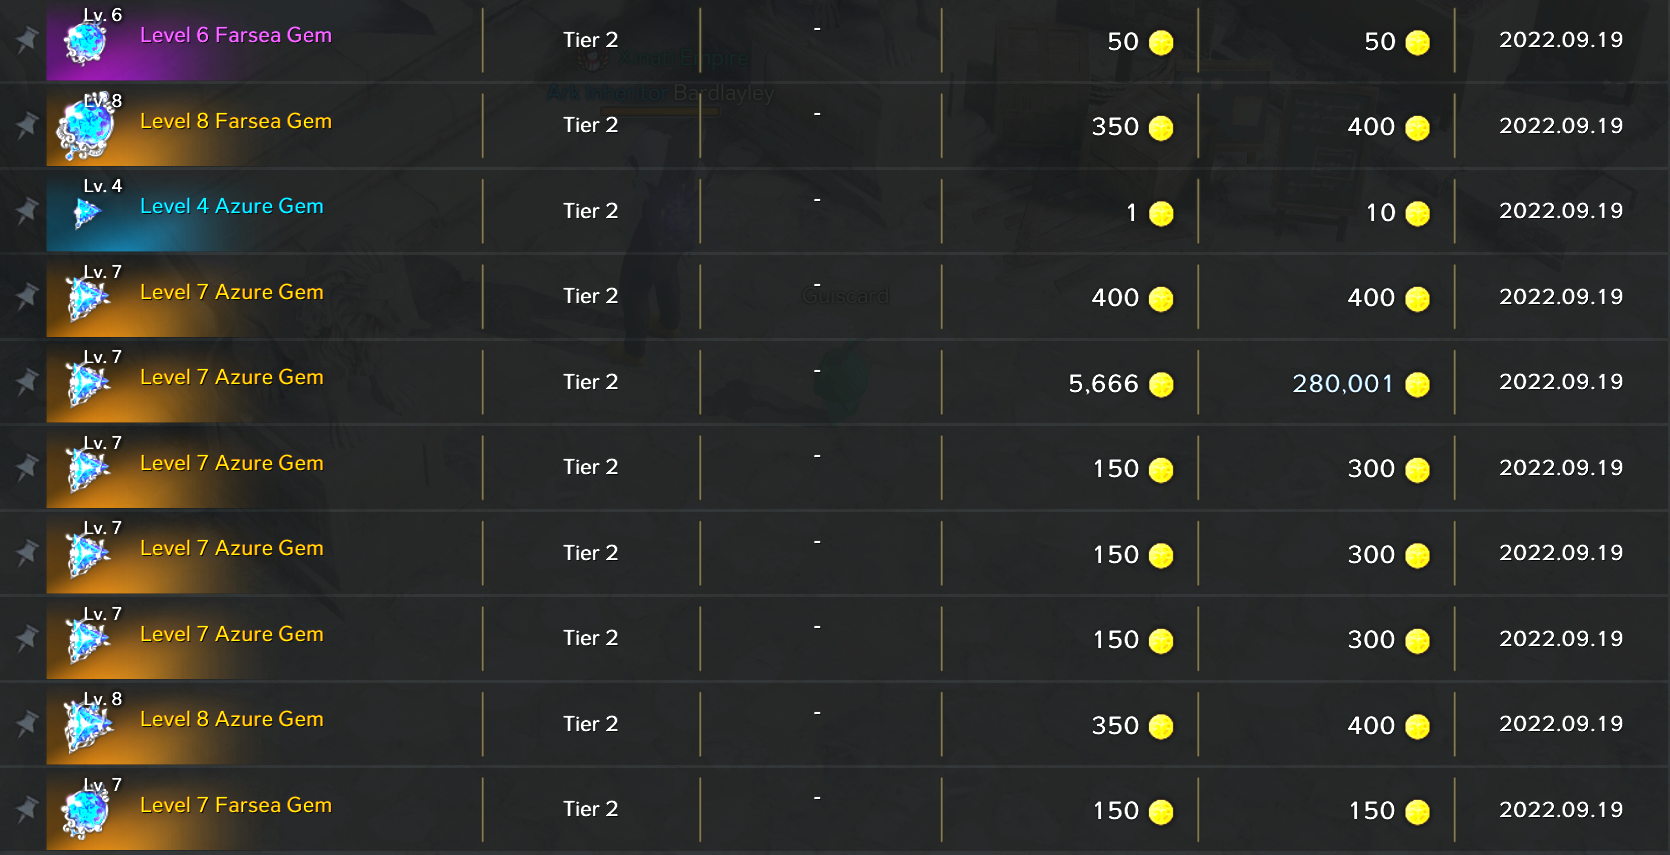
\includegraphics[scale=0.125]{auction-house-before}
    \caption{Auction house screenshot before image processing.}
    \label{figure:auction-house-before}
\end{figure}

\begin{figure}[H]
    \centering
    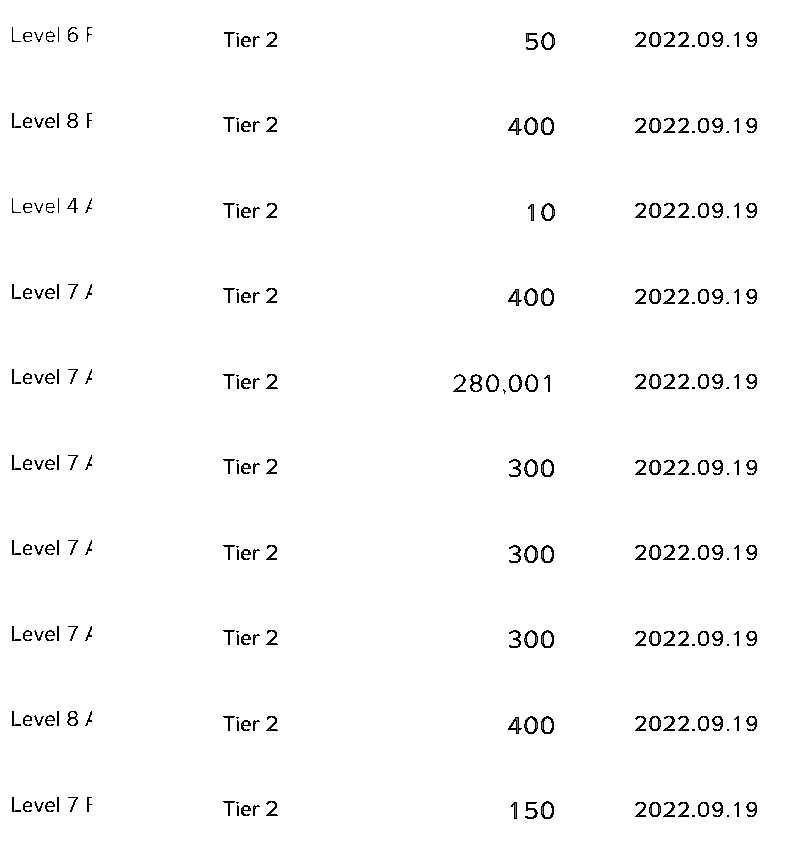
\includegraphics[scale=0.25]{auction-house-after}
    \caption{Auction house screenshot after image processing.}
    \label{figure:auction-house-after}
\end{figure}

\section{Validation and Verification}
\noindent Without having a labelled dataset, it will be difficult to accurately verify anomalous transactions using an algorithm. However, by utilising different algorithms for the testing of data, it is possible to check overlapping anomalies between different algorithms. This will allow for the verification that a data point is anomalous.

\subsection{Verifying Algorithms by Comparing Results of Different Algorithms}
\noindent Comparing the results is a way in which the data can be validated. By assigning each gem with a unique value based on its location within the database we can check each gem for its occurrence as an anomaly across multiple algorithms. An example in Python would look like this:
\lstinputlisting[language=python]{algorithms/compare-algorithms.py}

This method, however, suffers from a problem where anomalies which aren't detected by any algorithm won't be verified at all, leading to a reduced accuracy rate.

\section{Research Methodolody}

\section{Considerations}
\subsection{Legal}
\noindent 

\subsection{Ethical}
\noindent This paper follows the Nuremberg Code\cite{Nuremberg1947}.
The data being processed is gathered directly from the Lost Ark marketplace and doesn't contain any personally identifiable information which can be tied back to the user.

\subsection{Professional}
\noindent 

\section{Results and Analysis}
\noindent 

\section{Disccussion}
\noindent

\section{References Section}
\printbibliography

\begin{appendices}
    \section{Data Collection Code Samples}
    \label{appendix:collection-code}
    \subsection{image-formatter.py to turn auction house screenshots into OCR readable images.}
    \label{algorithm:image-formatter}
    \lstinputlisting[language=python]{algorithms/image-formatter.py}
    \subsection{image-processor.py to turn images into csv files based on the dataset date.}
    \label{algorithm:image-processor}
    \lstinputlisting[language=python]{algorithms/image-processor.py}
\end{appendices}

\end{document}